\section{Rilevazione degli eventi di Alternative Splicing}

\subsection{Descrizione generale}

Il Rilevatore di Eventi di Alternative Splicing si occupa di rilevare tutti gli eventi indotti dalle read. Per fare questo, confronta gli introni noti (deducibili dal file gtf) con quelli \textit{novel} (deducibili dagli allineamenti in formato MEM); analizzando le differenze tra i due è possibile rilevare gli eventi di Alternative Splicing.

Trovare gli introni noti è semplice, in quanto nel file gtf sono riportati tutti gli esoni con le relative posizioni di inizio e fine: gli introni sono quindi rappresentati dalla porzione di genoma tra un esone e un altro. 

La rilevazione degli introni novel è invece più complessa, e utilizza i MEMs generati dello Splice-Aware Aligner. Preso un generico allineamento, esso può essere rappresentato da uno o più MEMs. Nel secondo caso viene calcolata la distanza tra di essi sia sul genoma che sul testo degli esoni; si considerano introni tutte le porzioni del genoma dove questi due valori differiscono.

\begin{figure}[h!]
	\centering
	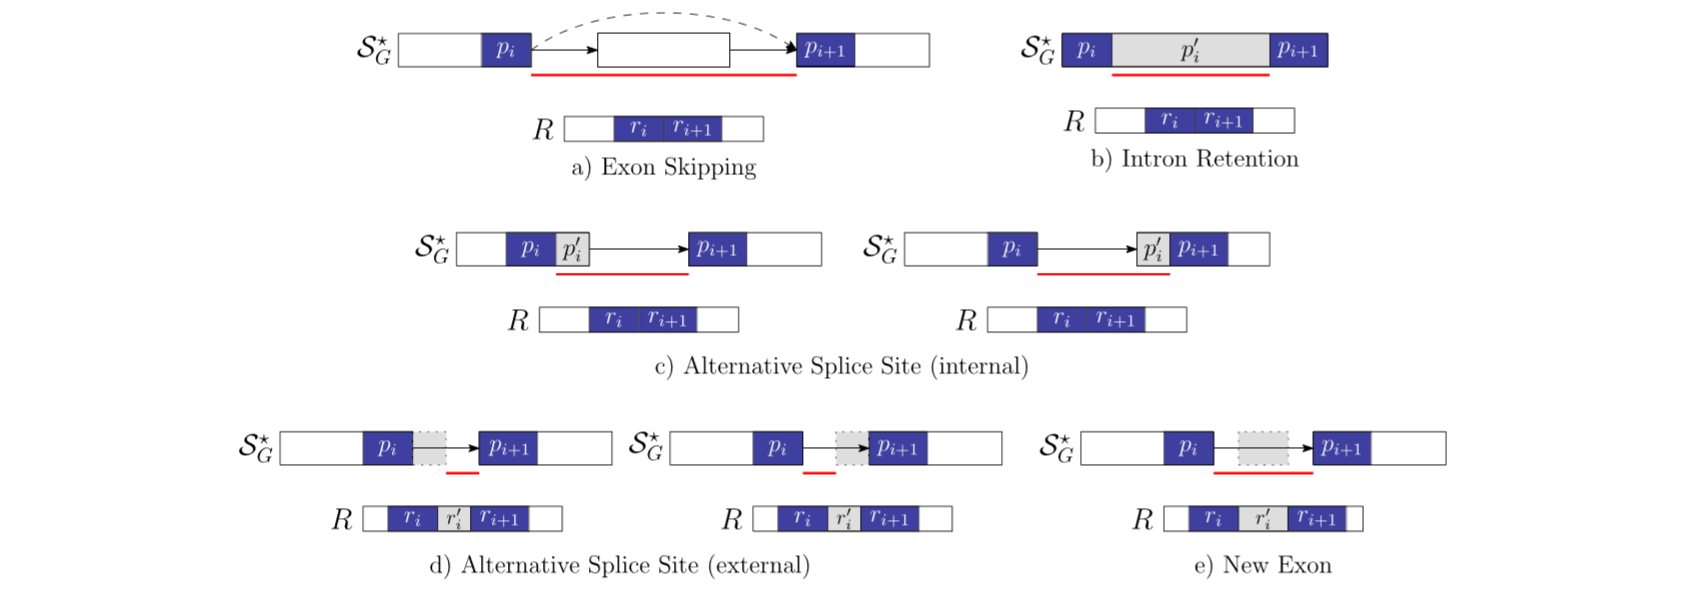
\includegraphics[width=\linewidth, height=7cm]{images/pattern.png}
  \caption{Fase di confronto degli introni}
  \label{fig:Summary}
\end{figure}

Viene poi eseguita una fase di riconciliazione (che permette di migliorare la qualità degli introni rilevati) e vengono filtrati quelli non supportati da un numero sufficiente di read.

A questo punto avviene la procedura di rilevazione vera e propria, che confronta gli introni novel con quelli noti, utilizzando dei pattern che rappresentano i vari eventi di Alternative Splicing.

La seguente immagine riassume la procedura:

\begin{figure}[h!]
	\centering
	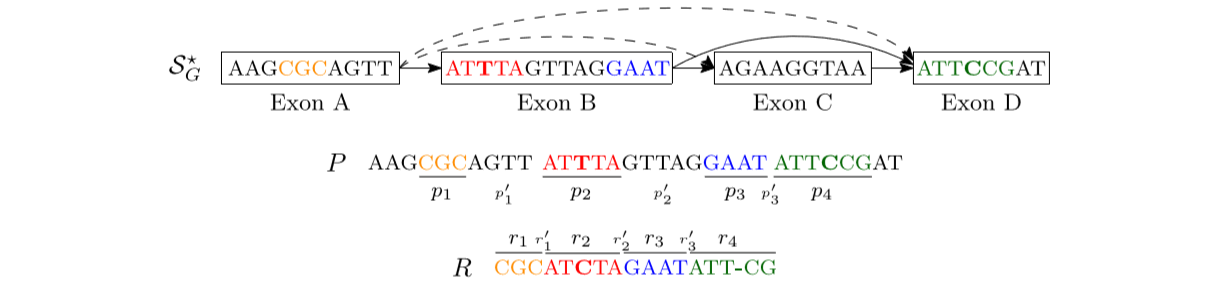
\includegraphics[width=\linewidth, height=5cm]{images/riassuntorilevazione.png}
  \caption{Riassunto della fase di rilevazione}
  \label{fig:Summary}
\end{figure}

\newpage

Gli eventi di Alternative Splicing così rilevati saranno poi riportati in un file \textit{.events.csv}, che contiene, per ogni evento rilevato:
\begin{enumerate}
	\item Il tipo di evento rilevato
	\item Le posizioni iniziali e finali sul genoma
	\item Il numero di read che supportano l'evento
	\item I transcritti che supportano l'evento
\end{enumerate}

\subsection{Merge degli introni dedotti dai due sample}

Come già detto in precedenza, i MEMs generati dallo Splice-Aware Aligner vengono utilizzati al fine di rilevare nuovi introni; ovviamente è necessario estendere questa procedura alle read paired-end. Si tratta in sostanza di fare una merge degli introni dedotti da ciascuno dei due file.

Il seguente frammento di codice mostra la procedura:

\begin{figure}[h!]
	\centering
	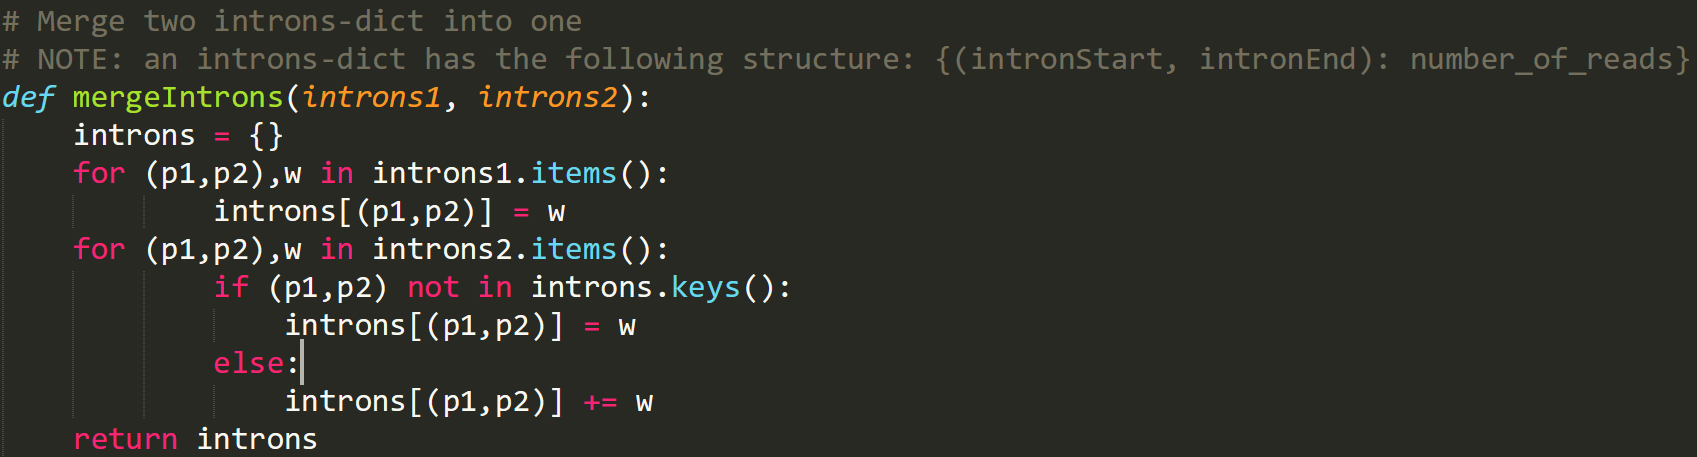
\includegraphics[width=\linewidth]{images/mergeIntrons.png}
  \label{fig:MergeIntrons}
\end{figure}


\newpage

\subsection{Calcolo dell' IDMP (Inner Distance between Mate Pairs)}
Considerando una coppia di read, si definisce IDMP (Inner Distance between Mate Pairs) la distanza sul genoma di riferimento in termini di BP (Base Pair) tra l'ultima base della prima read e la prima della seconda. Questa informazione viene generalmente fornita dall'ente che ha effettuato il sequenziamento, e può essere confrontata con l'IDMP rilevato durante l'allineamento per rilevare nuovi eventi di Alternative Splicing.

Visto che un allineamento può essere rappresentato da più di un MEM, non è possibile semplicemente aggiungere la lunghezza dell'allineamento alla sua posizione iniziale. Prima di poter calcolare l'IDMP è quindi necessario introdurre il concetto di BitVector, ovvero una sequenza di bit che rappresenta la posizione degli esoni nella genomica. Un BitVector è dotato di due operazioni:

\begin{itemize}
	\item Rank: data una posizione, ritorna l'esone di provenienza
	\item Select: dato un esone, ritorna la posizione di partenza 
\end{itemize}

Queste due operazioni permettono di calcolare l'IDMP in maniera efficace. Innanzitutto si prende l'ultimo MEM relativo all'allineamento della prima read, e si utilizza l'operazione di Rank per trovare l'esone di appartenenza. A questo punto, si utilizza l'operazione di Rank per trovare la posizione iniziale dell'esone. L'offset sarà quindi dato dalla differenza tra il MEM e la posizione iniziale dell'esone. Basta quindi aggiungere questo offset alla posizione iniziale per trovare la fine del primo allineamento.

% Sistemare, spiegare come viene calcolato.
L'inizio del secondo allineamento è noto. A questo punto basterà sottrarre ad esso la fine di quello precedente, in modo da ottenere l'IDMP.

Il seguente frammento di codice riassume la procedura:

\begin{figure}[h!]
	\centering
	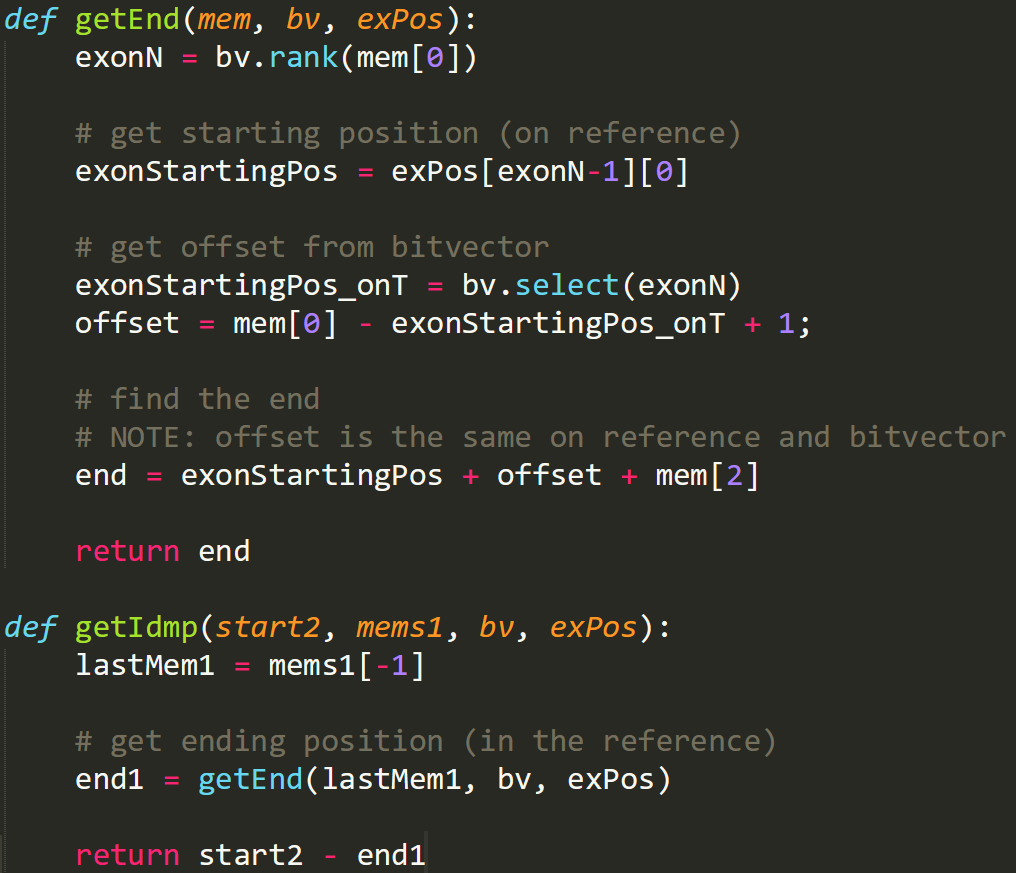
\includegraphics[width=\linewidth, height=9.5cm]{images/getIDMP.png}
  \label{fig:GetIDMP}
\end{figure}

\newpage

\subsection{Calcolo del TIDMP (Transcript-based IDMP)}
Per TIDMP si intende la misura della distanza \textit{sui trascritti} tra le due read. Per calcolarlo è innanzitutto necessario ottenere l'ultimo MEM relativo alla prima read e il primo MEM relativo alla seconda. Da ciascuno di essi è possibile ottenere la posizione iniziale e la lunghezza sul bitvector. A questo punto, usando l'operazione di rank, è possibile capire l'esone di provenienza di ciascun MEM.

Se i due MEM si trovano sullo stesso esone, il TIDMP è dato semplicemente dalla distanza tra la fine del primo MEM e l'inizio del secondo (sarà quindi uguale all' IDMP calcolato precedentemente).

Se i due MEM non si trovano sullo stesso esone, potrebbero essere su due esoni consecutivi o meno. Nel caso di esoni consecutivi, il TIDMP è dato dalla somma tra il suffisso non coperto dal primo esone e il prefisso non coperto dal secondo esone.

Il seguente frammento di codice mostra come calcolare il TIDMP:

\begin{figure}[h!]
	\centering
	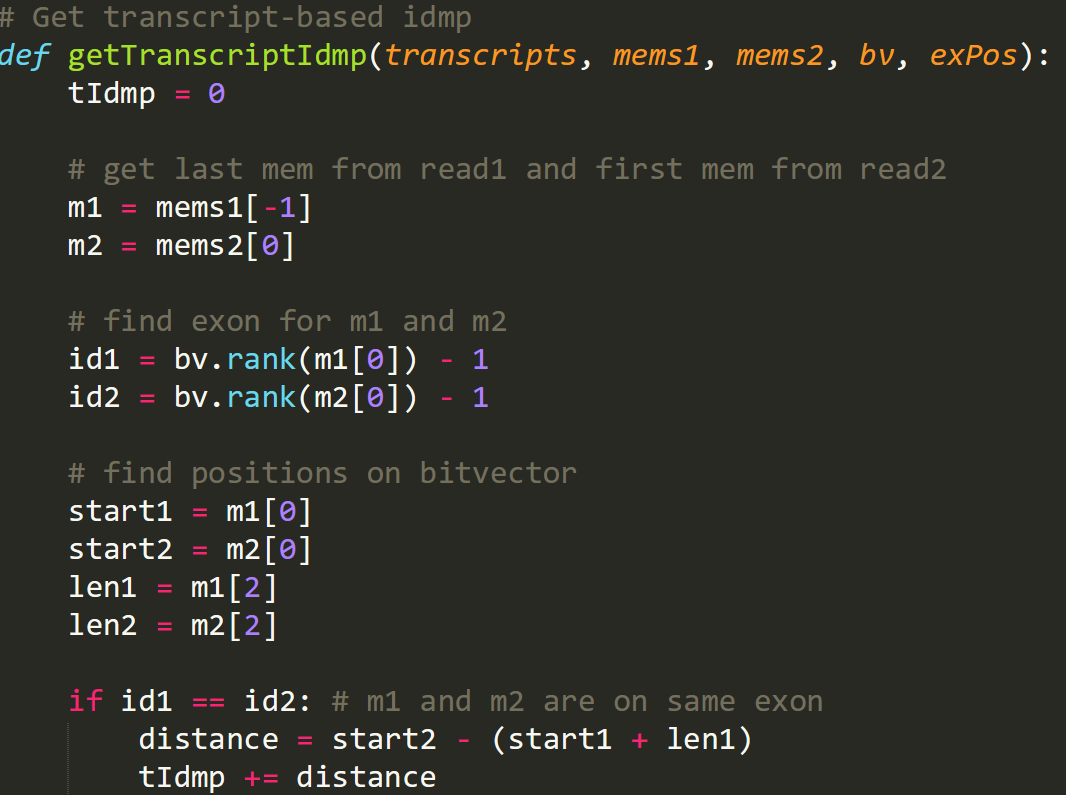
\includegraphics[width=\linewidth, height=9.5cm]{images/gettIDMP1.png}
  \label{fig:GettIDMP}
\end{figure}

\newpage

\begin{figure}[h!]
	\centering
	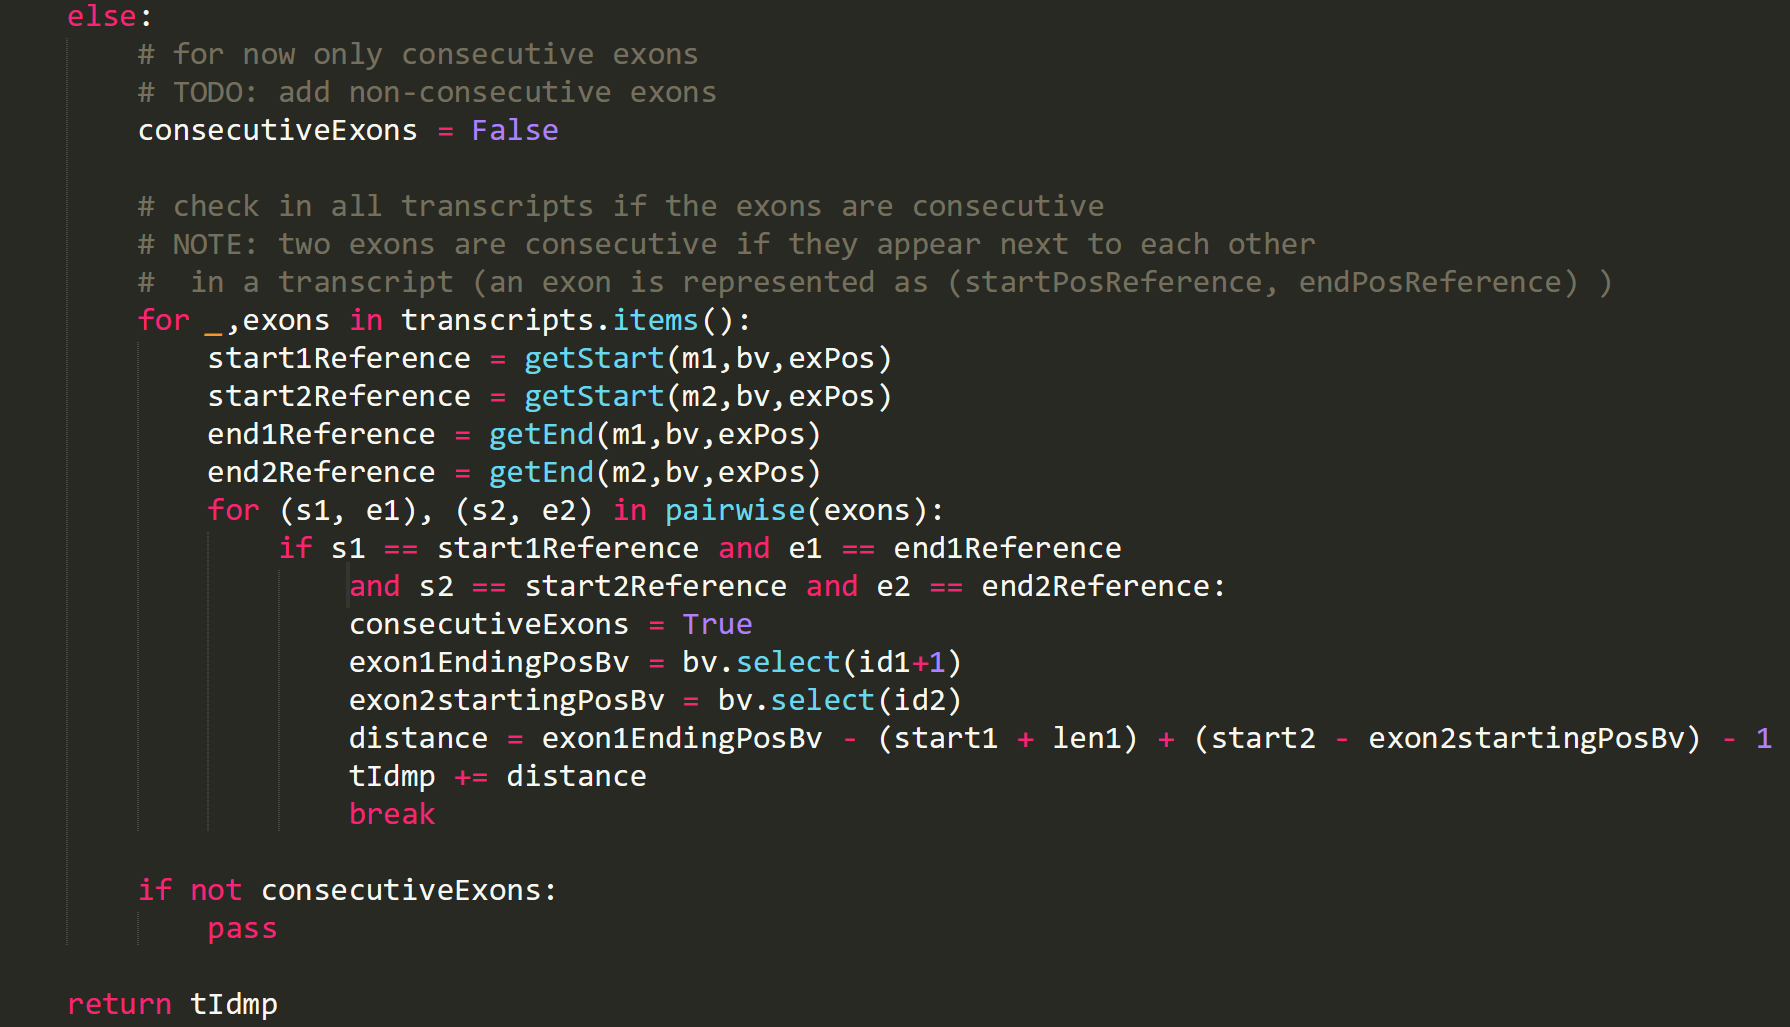
\includegraphics[width=\linewidth, height=9.5cm]{images/gettIDMP2.png}
  \label{fig:GettIDMP}
\end{figure}

Il caso di esoni non consecutivi presenta diverse criticità, e per il momento non è stato calcolato.

\newpage

\subsection{Possibile utilizzo di IDMP e TIDMP}

\newpage